\documentclass{article}
\usepackage{bm}
\usepackage{amsmath}
\usepackage{graphicx}
\usepackage{mdwlist}
\usepackage[colorlinks=true]{hyperref}
\usepackage{geometry}
\usepackage{kotex}
\geometry{margin=1in}
\geometry{headheight=2in}
\geometry{top=2in}
\usepackage{palatino}
%\renewcommand{\rmdefault}{palatino}
\usepackage{fancyhdr}
\usepackage{indentfirst}
\usepackage{multirow}
\usepackage{tabularx}

\newcommand{\red}[1]{{\color{red} #1}}
\newcommand{\blue}[1]{{\color{blue} #1}}
\newcommand{\orange}[1]{{\color{orange} #1}}
\newcommand{\purple}[1]{{\color{purple} #1}}

%\pagestyle{fancy}
\rhead{}
\lhead{}
\chead{%
  {\vbox{%
      \vspace{2mm}
      \large
      Statistics Lab 033.020\hfill
\\
      Seoul National University
      \\[4mm]
      \textbf{Assignment \#7} \\
      \texttt{2016-19516, Sangjun Son}
    }
  }
}

%%%%%%%%%%%%%%%%%%%%%%%
\usepackage{xcolor}
\usepackage{listings}
\definecolor{vgreen}{RGB}{104,180,104}
\definecolor{vblue}{RGB}{49,49,255}
\definecolor{vorange}{RGB}{255,143,102}

\lstdefinestyle{r-style}
{
    language=R,
    basicstyle=\footnotesize\ttfamily,
    keywordstyle=\color{vblue},
    identifierstyle=\color{black},
    commentstyle=\color{vgreen},
    numbers=left,
    numberstyle=\tiny\color{black},
    numbersep=10pt,
    tabsize=8,
    moredelim=*[s][\colorIndex]{[}{]},
    literate=*{:}{:}1,
    escapeinside=``,
}

\lstdefinestyle{out-style}
{
    basicstyle=\footnotesize\ttfamily,
    numbersep=10pt,
    tabsize=8,
    moredelim=*[s][\colorIndex]{[}{]},
    literate=*{:}{:}1,
    escapeinside=``,
}

\makeatletter
\newcommand*\@lbracket{[}
\newcommand*\@rbracket{]}
\newcommand*\@colon{:}
\newcommand*\colorIndex{%
    \edef\@temp{\the\lst@token}%
    \ifx\@temp\@lbracket \color{black}%
    \else\ifx\@temp\@rbracket \color{black}%
    \else\ifx\@temp\@colon \color{black}%
    \else \color{vorange}%
    \fi\fi\fi
}
\makeatother

\usepackage{trace}
%%%%%%%%%%%%%%%%%%%%%%%

\usepackage{paralist}

\usepackage{todonotes}
\setlength{\marginparwidth}{2.15cm}

\usepackage{tikz}
\usetikzlibrary{positioning,shapes,backgrounds}

\begin{document}

\pagestyle{fancy}

\section*{Example 1}
(\texttt{handspan.txt}) 다음은 167명의 학생들에 대해 성별 (Sex)과 신장 (Height) 그리고 손 한뼘의 길이 (HandSpan)를 측정한 자료이다.\\

\textbf{(1)} 신장과 손 한뼘의 길이는 서로 상관관계가 존재하는가? 표본 상관계수를 구하고 두 변수의 산점도를 그려보자. 두 변수 사이에 선형적 연관성이 존재하는가?

\begin{lstlisting}[style={r-style}]
handspan = read.table("handspan.txt", header=T)
plot(handspan$Height, handspan$HandSpan)
cor(handspan$Height, handspan$HandSpan)
\end{lstlisting}
\begin{lstlisting}[style={out-style}]
[1] 0.7395375
\end{lstlisting}
\begin{figure}[htb!]
    \centering
    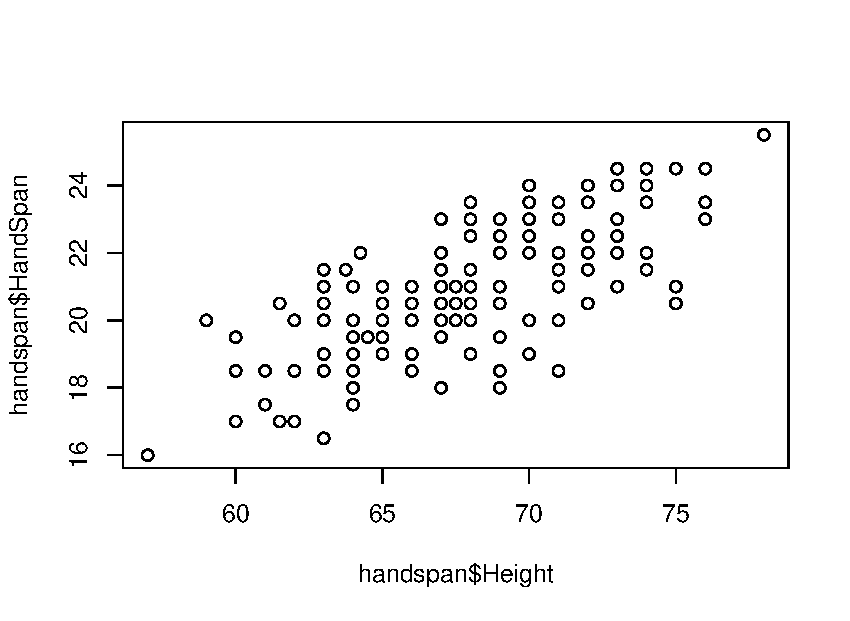
\includegraphics[width=0.6\textwidth]{fig/ex1-1.pdf}
\end{figure}
\emph{Explanation: 먼저 두 변수에 대한 상관계수를 cor()를 통해 구해보면 0.7395로 나타나고 plot()을 이용하여 그린 산점도 상으로 두 변수 간에는 어느 정도 선형적 연관성이 있음을 확인할 수 있다. } \\

\textbf{(2)} 신장과 손 한뼘의 길이사이에 상관관계가 존재하는지 유의수준 5\%에서 검정하여라.

\begin{lstlisting}[style={r-style}]
cor.test(handspan$Height, handspan$HandSpan)
\end{lstlisting}
\begin{lstlisting}[style={out-style}]
---------------------------------------------------------------------------------------
	Pearson's product-moment correlation

data:  handspan$Height and handspan$HandSpan
t = 14.113, df = 165, p-value < 2.2e-16
alternative hypothesis: true correlation is not equal to 0
95 percent confidence interval:
 0.6620252 0.8013971
sample estimates:
      cor 
0.7395375 
---------------------------------------------------------------------------------------
\end{lstlisting}
\emph{Explanation: 상관관계의 유무에 대한 검정은 cor.test() 함수를 사용해서 시행할 수 있다. 상관관계 유무의
검정 결과, 검정통계량은 14.113이고 유의확률은 매우 작은 것으로 확인되었다. 따라서 유의수준 5\%에서 두 변수 (Height, HandSpan) 사이의 상관관계가 존재한다는 매우 뚜렷한 증거가 있다.} \\

\textbf{(3)} 신장 (y)과 손 한뼘의 길이 (x)에 대해 단순선형회귀모형을 적용해보자. 추정된 회귀식을 구하고 유의수준 5\%에서 회귀 직선의 유의성을 검정하시오.

\begin{lstlisting}[style={r-style}]
handspan.res <- lm(handspan$Height ~ handspan$HandSpan); handspan.res
summary(handspan.res)
anova(handspan.res)
\end{lstlisting}
\begin{lstlisting}[style={out-style}]
---------------------------------------------------------------------------------------
Call:
lm(formula = handspan$Height ~ handspan$HandSpan)

Coefficients:
      (Intercept)  handspan$HandSpan  
            35.53               1.56  
---------------------------------------------------------------------------------------
Call:
lm(formula = handspan$Height ~ handspan$HandSpan)

Residuals:
    Min      1Q  Median      3Q     Max 
-7.7266 -1.7266 -0.1666  1.4933  7.4933 

Coefficients:
                  Estimate Std. Error t value Pr(>|t|)    
(Intercept)        35.5250     2.3160   15.34   <2e-16 ***
handspan$HandSpan   1.5601     0.1105   14.11   <2e-16 ***
---
Signif. codes:  
0 '***' 0.001 '**' 0.01 '*' 0.05 '.' 0.1 ' ' 1

Residual standard error: 2.744 on 165 degrees of freedom
Multiple R-squared:  0.5469,	Adjusted R-squared:  0.5442 
F-statistic: 199.2 on 1 and 165 DF,  p-value: < 2.2e-16
---------------------------------------------------------------------------------------
Analysis of Variance Table

Response: handspan$Height
                   Df Sum Sq Mean Sq F value    Pr(>F)    
handspan$HandSpan   1 1500.1 1500.06  199.17 < 2.2e-16 ***
Residuals         165 1242.7    7.53                      
---
Signif. codes:  
0 '***' 0.001 '**' 0.01 '*' 0.05 '.' 0.1 ' ' 1
---------------------------------------------------------------------------------------
\end{lstlisting}
\emph{Explanation: \\
(1) 회귀식의 적합은 lm() 함수를 사용할 수 있다. lm() 함수 안에 선형회귀식의 독립변수 ($x$ : HandSpan)와 종속변수 ($y$ : Height)를 다음과 같이 입력한다. 실행 결과, $\textbf{y = 35.53 + 1.56x}$의 추정 회귀식을 구할 수 있었다. \\
(2) summary()를 통한 회귀 계수의 유의성
검정 결과, 설명변수 HandSpan의 $t$-검정 통계량의 값은 15.34로써 유의확률은 매우 작다. 
결정계수 (Multiple R-squared)는 0.5469으로써 전체 자료의 산포 중 약 54.69\%가 회귀직선으로 설명이 가능한 것을 알 수 있다. 
회귀모형의 유의성 검정 결과인 $F$-검정 통계량의 값은
199.2이고 유의확률은 매우 작은 것으로 나타났다. \textbf{따라서 유의수준 5\%에서 회귀직선은 유의하다고 말할 수 있다.}  \\
(3) anova()를 통해 적합된 회귀 모형의 분산분석표를 출력하였고 결과는 summary()에서 출력되는 $F$-검정 통계량과 동일한 것을 볼 수 있다.} \\

\textbf{(4)} 단순 선형 회귀모형의 적용은 타당한가? 잔차도를 이용하여 답하시오.

\begin{lstlisting}[style={r-style}]
par(mfrow=c(1,2))
plot(handspan.res)
dev.off()
\end{lstlisting}
\begin{figure}[htb!]
    \centering
    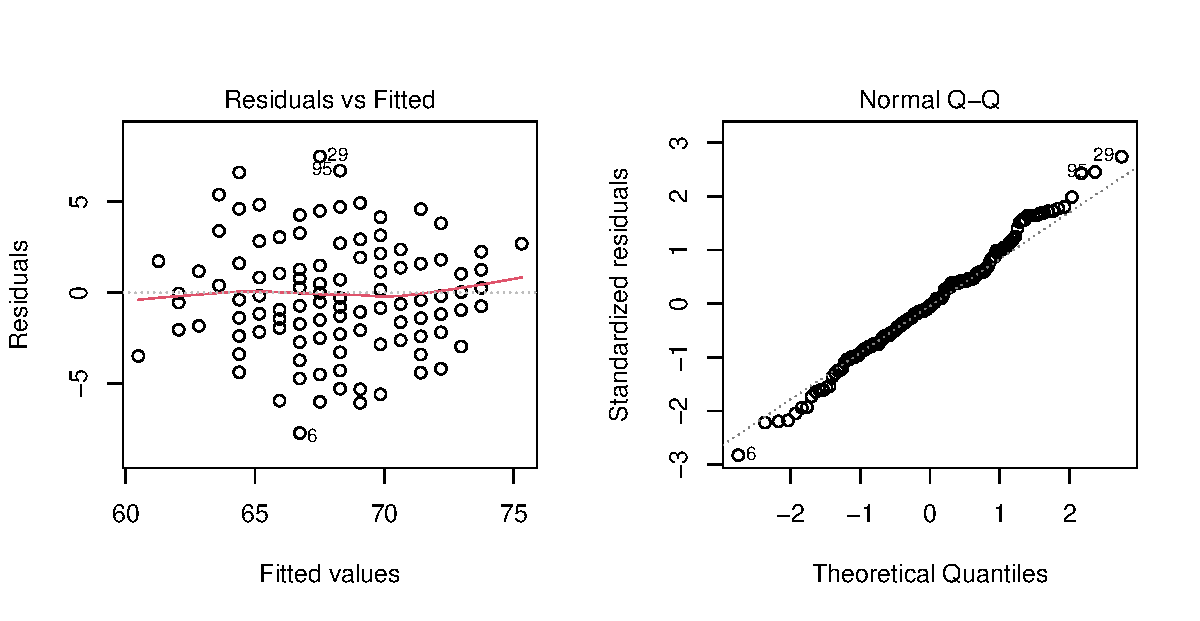
\includegraphics[width=1.0\textwidth]{fig/ex1-4.pdf}
\end{figure}
\emph{Explanation: 적합한 회귀분석의 결과는 handspan.res 에 저장되어 있다. 적합된 결과에 대한 잔차도를 plot() 함수를 이용해서 출력한 결과, 잔차들은 (a) \textbf{선형성}, (b) \textbf{독립성}: 특정한 패턴을 보이거나 (c) \textbf{등분산성}: 분산의 분포가 일정한 것으로 보아 가정을 위배한 것으로 보이지 않는다. 하지만 몇몇 잔차의 경우 범위를 벗어난 큰 값을 갖는 것으로 확인된다. 정규 분위수 그래프를 확인해 보면 양 끝쪽으로 직선에서 벗어난 점들이 관찰되는데 대부분의 잔차는 (d) \textbf{정규성}: 직선 주위에 몰려있는 것을 확인할 수 있다. 따라서 단순선형회귀모형의 적용은 타당함을 알 수 있다.} \\

\newpage
\section*{Example 2}
(\texttt{carstopping.txt}) 주어진 자료는 브레이크가 작동되는 순간의 자동차의 주행 속도 (Speed)에 따른 자동차 제동 거리 (StopDist)를 조사한 자료이다. \\

\textbf{(1)} 자동차의 주행 속도에 따른 자동차의 제동거리 간에는 서로 상관관계가 존재하는가? 상관분석을 통해 이를 확인해보자.

\begin{lstlisting}[style={r-style}]
carstopping = read.table("carstopping.txt", header=T)
plot(carstopping$Speed, carstopping$StopDist)
cor.test(carstopping$Speed, carstopping$StopDist)
\end{lstlisting}
\begin{lstlisting}[style={out-style}]
---------------------------------------------------------------------------------------
	Pearson's product-moment correlation

data:  carstopping$Speed and carstopping$StopDist
t = 20.68, df = 61, p-value < 2.2e-16
alternative hypothesis: true correlation is not equal to 0
95 percent confidence interval:
 0.8952425 0.9606129
sample estimates:
      cor 
0.9355037 
---------------------------------------------------------------------------------------
\end{lstlisting}
\begin{figure}[htb!]
    \centering
    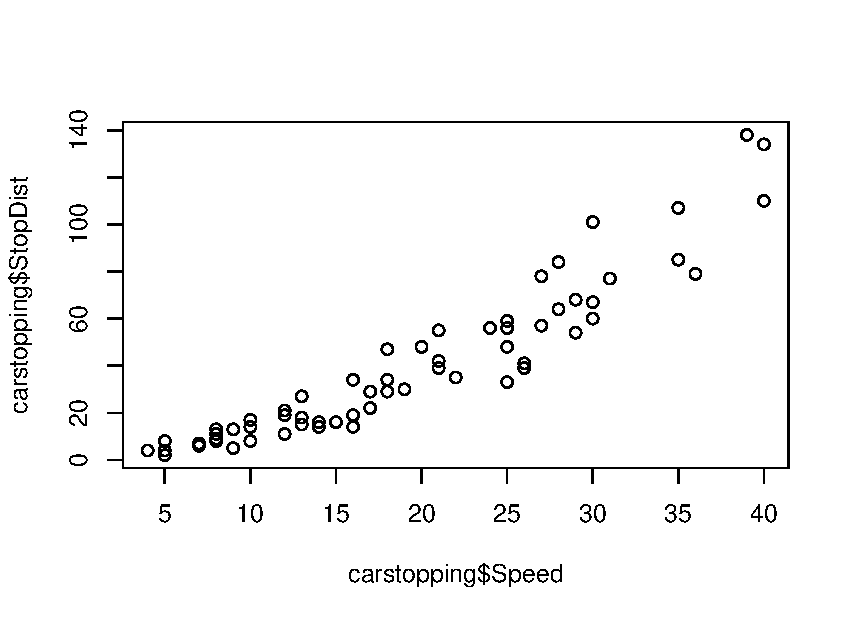
\includegraphics[width=0.6\textwidth]{fig/ex2-1.pdf}
\end{figure}
\emph{Explanation: 먼저 plot()을 이용하여 두 변수 간의 상관관계를 그리고 만들어진 산점도 상으로 두 변수 간에는 어느 정도 선형적 연관성이 있음을 확인할 수 있다. cor.test()를 통한 상관관계 유무의
검정 결과, 상관계수는 0.9055와 검정통계량은 20.68이고 유의확률은 매우 작은 것으로 확인되었다. 따라서 유의수준 5\%에서 두 변수 자동차의 주행 속도 (Speed)에 따른 자동차 제동 거리 (StopDist) 사이의 상관관계가 존재한다는 매우 뚜렷한 증거가 있다.} \\

\textbf{(2)} 주어진 자료에 단순 선형회귀모형을 적용한 후 결과를 확인해 보자. 유의수준 5\%에서 모형은 유의한가? 

\begin{lstlisting}[style={r-style}]
carstopping.res <- lm(carstopping$StopDist ~ carstopping$Speed); carstopping.res
summary(carstopping.res)
anova(carstopping.res)
\end{lstlisting}
\begin{lstlisting}[style={out-style}]
---------------------------------------------------------------------------------------
Call:
lm(formula = carstopping$StopDist ~ carstopping$Speed)

Coefficients:
      (Intercept)  carstopping$Speed  
          -20.273              3.137  
---------------------------------------------------------------------------------------
Call:
lm(formula = carstopping$StopDist ~ carstopping$Speed)

Residuals:
    Min      1Q  Median      3Q     Max 
-25.141  -7.300  -2.141   6.044  35.946 

Coefficients:
                  Estimate Std. Error t value Pr(>|t|)    
(Intercept)       -20.2734     3.2384   -6.26 4.25e-08 ***
carstopping$Speed   3.1366     0.1517   20.68  < 2e-16 ***
---
Signif. codes:  
0 '***' 0.001 '**' 0.01 '*' 0.05 '.' 0.1 ' ' 1

Residual standard error: 11.8 on 61 degrees of freedom
Multiple R-squared:  0.8752,	Adjusted R-squared:  0.8731 
F-statistic: 427.7 on 1 and 61 DF,  p-value: < 2.2e-16
---------------------------------------------------------------------------------------
Analysis of Variance Table

Response: carstopping$StopDist
                  Df Sum Sq Mean Sq F value    Pr(>F)    
carstopping$Speed  1  59540   59540  427.65 < 2.2e-16 ***
Residuals         61   8493     139                      
---
Signif. codes:  
0 '***' 0.001 '**' 0.01 '*' 0.05 '.' 0.1 ' ' 1
---------------------------------------------------------------------------------------
\end{lstlisting}
\emph{Explanation:  \\
(1) 회귀식 적합을 위해 lm() 안에 선형회귀식의 독립변수 ($x$ : Speed)와 종속변수 ($y$ : StopDist)를 매개변수로 한 뒤, 실행 결과, $\textbf{y = -20.273 + 3.137x}$의 추정 회귀식을 구할 수 있었다. \\
(2) summary()를 통한 회귀 계수의 유의성
검정 결과, 설명변수 HandSpan의 $t$-검정 통계량의 값은 20.68로써 유의확률은 매우 작다. 
결정계수 (Multiple R-squared)는 0.8752으로써 전체 자료의 산포 중 약 87.52\%가 회귀직선으로 설명이 가능한 것을 알 수 있다. 
회귀모형의 유의성 검정 결과인 $F$-검정 통계량의 값은
427.7이고 유의확률은 매우 작은 것으로 나타났다. \textbf{따라서 유의수준 5\%에서 회귀직선은 유의하다고 말할 수 있다.}  \\
(3) anova()를 통해 적합된 회귀 모형의 분산분석표를 출력하였고 결과는 summary()에서 출력되는 $F$-검정 통계량과 동일한 것을 볼 수 있다.} \\

\textbf{(3)} 적합된 회귀 모형의 잔차도를 확인해 보자. 단순선형회귀모형의 적용이 타당하다고 볼 수 있는가?

\begin{lstlisting}[style={r-style}]
par(mfrow=c(1,2))
plot(carstopping.res)
dev.off()
\end{lstlisting}
\begin{figure}[htb!]
    \centering
    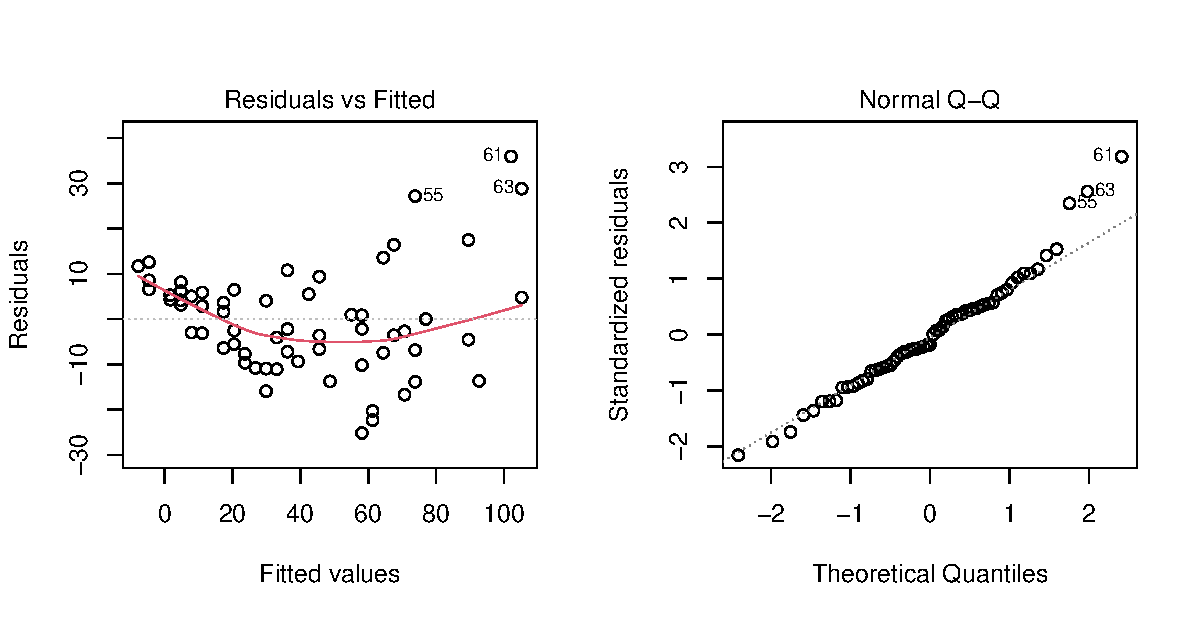
\includegraphics[width=1.0\textwidth]{fig/ex2-3.pdf}
\end{figure}
\emph{Explanation: 적합한 회귀분석의 결과는 carstopping.res 에 저장되어 있다. 적합된 결과에 대한 잔차도를 plot() 함수를 이용해서 출력한 결과, 잔차들은 (a) \textbf{선형성}, (b) \textbf{독립성}: 특정한 패턴을 보이거나 (c) \textbf{등분산성}: 분산의 분포가 일정한 것으로 보아 가정을 위배한 것으로 보이지 않는다. 하지만 몇몇 잔차의 경우 범위를 벗어난 큰 값을 갖는 것으로 확인된다. 정규 분위수 그래프를 확인해 보면 양 끝쪽으로 직선에서 벗어난 점들이 관찰되는데 대부분의 잔차는 (d) \textbf{정규성}: 직선 주위에 몰려있는 것을 확인할 수 있다. 따라서 단순선형회귀모형의 적용은 타당함을 알 수 있다.} \\

\section*{Example 3}
(\texttt{hospital.txt}) 다음은 미국 내 113개의 병원들을 대상으로 입원 기간 동안 환자들이 받는 감염 위험과 관련된 사항들을 조사하였다. 다음은 주요 변수에 대한 설명이다. 
\begin{table}[htb!]
\centering
\begin{tabular}{|c|l|}
\hline
변수명 & 설명 \\ \hline
\texttt{InfctRsk} & 종속변수. 감염 위험 정도 \\ \hline
\texttt{Stay} & 설명변수1. 환자들의 평균 입원 기간 \\ \hline
\texttt{Age} & 설명변수2. 환자들의 평균 나이 \\ \hline
\texttt{Xray} & 설명변수3. 해당 병원의 X-ray 검진 횟수 \\ \hline
\end{tabular}
\end{table}

\textbf{(1)} 종속변수와 각 설명변수들 간에는 유의한 상관관계가 존재하는가? 산점도와 상관분석을
통해 이를 확인해보시오.

\begin{lstlisting}[style={r-style}]
hospital = read.table("hospital.txt", header=T)

par(mfrow=c(1,3))
plot(InfctRsk ~ Stay + Age + Xray, data=hospital)
cor.test(hospital$InfctRsk, hospital$Stay)
cor.test(hospital$InfctRsk, hospital$Age)
cor.test(hospital$InfctRsk, hospital$Xray)
dev.off()
\end{lstlisting}
\begin{lstlisting}[style={out-style}]
---------------------------------------------------------------------------------------
	Pearson's product-moment correlation

data:  hospital$InfctRsk and hospital$Stay
t = 6.6445, df = 111, p-value = 1.177e-09
alternative hypothesis: true correlation is not equal to 0
95 percent confidence interval:
 0.3868338 0.6537511
sample estimates:
      cor 
0.5334438 
---------------------------------------------------------------------------------------
	Pearson's product-moment correlation

data:  hospital$InfctRsk and hospital$Age
t = 0.011517, df = 111, p-value = 0.9908
alternative hypothesis: true correlation is not equal to 0
95 percent confidence interval:
 -0.1836737  0.1857855
sample estimates:
        cor 
0.001093166 
---------------------------------------------------------------------------------------
	Pearson's product-moment correlation

data:  hospital$InfctRsk and hospital$Xray
t = 5.3593, df = 111, p-value = 4.585e-07
alternative hypothesis: true correlation is not equal to 0
95 percent confidence interval:
 0.2932204 0.5888060
sample estimates:
      cor 
0.4533916
---------------------------------------------------------------------------------------
\end{lstlisting}
\begin{figure}[htb!]
    \centering
    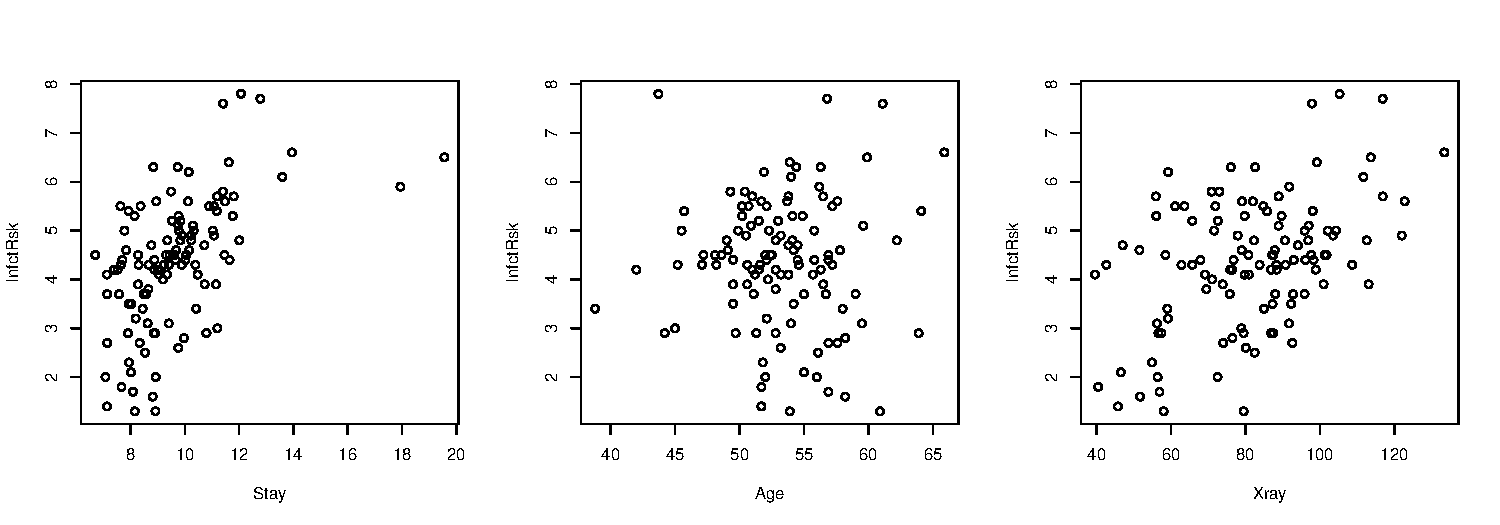
\includegraphics[width=1.0\textwidth]{fig/ex3-1.pdf}
\end{figure}
\emph{Explanation: 먼저 plot()을 이용하여 두 변수 간의 상관관계를 그린다. 종속변수 (InfctRsk)를 설명하는데 다양한 변수들이 존재하므로 각각의 산점도를 모든 쌍에 대해 그려야 하며 마찬가지로 상관관계 유무에 대한 검정도 쌍으로 진행해야 한다. 만들어진 산점도 상으로 \textbf{(InfctRsk, Stay)와 (InfctRsk, Xray) 끼리는 어느 정도 선형적 연관성이 있음을 확인할 수 있으나 (InfctRsk, Age)는 있다고 할 수 있는 뚜렷한 모양이 보이지 않았다.} \\ cor.test()를 통한 상관관계 유무의 검정 결과, InfctRsk와 Stay/Age/Xray에 대한 각각의 상관계수는 0.53/0.00/0.45으로 나타났으며 검정통계량은 6.64/0.01/5.36으로 확인되었다. \textbf{따라서 유의수준 5\%에서 종속변수 감염 위험 정도 (InfctRsk)는 두 가지 설명변수 환자들의 평균 입원 기간 (Stay)과 해당 병원의 X-ray 검진 횟수 (Xray)는 상관관계가 있다고 할 수 있지만 Age (환자들의 평균 나이)와 상관있다는 뚜렷한 증거가 없다.}} \\

\textbf{(2)} 주어진 자료에 다중선형회귀모형을 적용해보자. 유의수준 5\%에서 모형은 유의하다고 할
수 있는가? 각 변수들은 유의한가?

\begin{lstlisting}[style={r-style}]
hospital.res <- lm(InfctRsk ~ Stay + Age + Xray, data=hospital); hospital.res
summary(hospital.res)
anova(hospital.res)
\end{lstlisting}
\begin{lstlisting}[style={out-style}]
---------------------------------------------------------------------------------------
Call:
lm(formula = InfctRsk ~ Stay + Age + Xray, data = hospital)

Coefficients:
(Intercept)         Stay          Age         Xray  
    1.00116      0.30818     -0.02301      0.01966  
---------------------------------------------------------------------------------------
Call:
lm(formula = InfctRsk ~ Stay + Age + Xray, data = hospital)

Residuals:
     Min       1Q   Median       3Q      Max 
-2.77320 -0.73779 -0.03345  0.73308  2.56331 

Coefficients:
             Estimate Std. Error t value Pr(>|t|)    
(Intercept)  1.001162   1.314724   0.761 0.448003    
Stay         0.308181   0.059396   5.189 9.88e-07 ***
Age         -0.023005   0.023516  -0.978 0.330098    
Xray         0.019661   0.005759   3.414 0.000899 ***
---
Signif. codes:  
0 '***' 0.001 '**' 0.01 '*' 0.05 '.' 0.1 ' ' 1

Residual standard error: 1.085 on 109 degrees of freedom
Multiple R-squared:  0.363,	Adjusted R-squared:  0.3455 
F-statistic:  20.7 on 3 and 109 DF,  p-value: 1.087e-10
---------------------------------------------------------------------------------------
Analysis of Variance Table

Response: InfctRsk
           Df  Sum Sq Mean Sq F value    Pr(>F)    
Stay        1  57.305  57.305 48.6920 2.444e-10 ***
Age         1   2.075   2.075  1.7632 0.1870031    
Xray        1  13.719  13.719 11.6568 0.0008992 ***
Residuals 109 128.281   1.177                      
---
Signif. codes:  
0 '***' 0.001 '**' 0.01 '*' 0.05 '.' 0.1 ' ' 1
---------------------------------------------------------------------------------------
\end{lstlisting}
\emph{Explanation: \\
(1) 회귀식 적합을 위해 lm() 안에 선형회귀식의 독립변수 ($x1$ : Stay, $x2$ : Age, $x3$ : Xray)와 종속변수 ($y$ : InfctRsk)를 매개변수로 한 뒤, 실행 결과, $\textbf{y = 1.00116 + 0.30818 x1 - 0.02301 x2 + 0.01966 x3}$의 추정 회귀식을 구할 수 있었다. \\
(2) summary()를 통한 회귀 계수의 유의성 검정 결과, 독립변수 Stay, Xray의 검정에 대한 유의확률은 매우 작으나, Age의 경우 0.330098로 유의하다고 볼 수 없다. 하지만 회귀모형의 유의성 검정 결과인 $F$-검정 통계량의 값은
20.7로 유의확률 또한 매우 작은 것으로 나타났다. \textbf{따라서 유의수준 5\%에서 회귀직선은 유의하다고 말할 수 있다. 하지만 Stay, Xray 변수는 유의한 반면, Age 변수는 유의하지 않음을 확인하였다.}  \\
(3) anova()를 통해 적합된 회귀 모형의 분산분석표를 출력하였고 결과는 summary()에서 출력되는 $F$-검정 통계량과 동일한 것을 볼 수 있다.} \\

\textbf{(3)} 다중선형회귀모형의 적용은 타당하다고 볼 수 있는가?

\begin{lstlisting}[style={r-style}]
par(mfrow=c(1,2))
plot(hospital.res)
dev.off()
\end{lstlisting}
\begin{figure}[htb!]
    \centering
    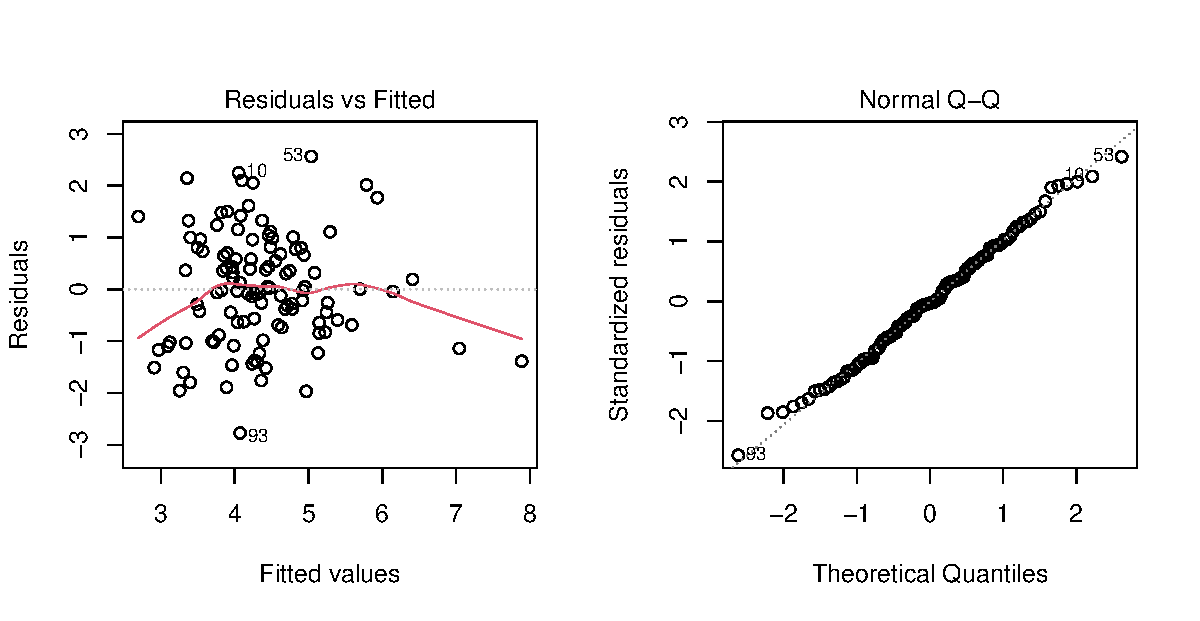
\includegraphics[width=1.0\textwidth]{fig/ex3-3.pdf}
\end{figure}
\emph{Explanation: 적합한 회귀분석의 결과는 hospital.res 에 저장되어 있다. 적합된 결과에 대한 잔차도를 plot() 함수를 이용해서 출력한 결과, 잔차들은 (a) \textbf{선형성}, (b) \textbf{독립성}: 특정한 패턴을 보이거나 (c) \textbf{등분산성}: 분산의 분포가 일정한 것으로 보아 가정을 위배한 것으로 보이지 않는다. 하지만 몇몇 잔차의 경우 범위를 벗어난 큰 값을 갖는 것으로 확인된다. 정규 분위수 그래프를 확인해 보면 양 끝쪽으로 직선에서 벗어난 점들이 관찰되는데 대부분의 잔차는 (d) \textbf{정규성}: 직선 주위에 몰려있는 것을 확인할 수 있다. 따라서 단순선형회귀모형의 적용은 타당함을 알 수 있다.} \\

\section*{Example 4}
(\texttt{hospital.txt}) 예제 3에서 종속변수 (InfctRsk)를 설명하는데 Age 변수는 유의하지 않음을
확인하였다. 이에 Age 변수를 제외하고 나머지 2개의 설명변수 (Stay, Xray)만을 이용하여 다중선형회귀모형을 적용해보고자 한다. \\

\textbf{(a)} 주어진 자료에 다중선형회귀모형을 적용해보자. 유의수준 5\%에서 모형은 유의하다고
말할 수 있는가? 새로운 모형의 $R^2$와 $adjusted \ R^2$를 구하고, 예제 3에서 구한 값과 각각 비교하여라.

\begin{lstlisting}[style={r-style}]
hospital.res <- lm(InfctRsk ~ Stay + Xray, data=hospital); hospital.res
summary(hospital.res)
anova(hospital.res)
\end{lstlisting}
\begin{lstlisting}[style={out-style}]
---------------------------------------------------------------------------------------
Call:
lm(formula = InfctRsk ~ Stay + Xray, data = hospital)

Coefficients:
(Intercept)         Stay         Xray  
   -0.15060      0.29584      0.02023
---------------------------------------------------------------------------------------
Call:
lm(formula = InfctRsk ~ Stay + Xray, data = hospital)

Residuals:
     Min       1Q   Median       3Q      Max 
-2.79635 -0.71592 -0.01511  0.73899  2.39483 

Coefficients:
             Estimate Std. Error t value Pr(>|t|)    
(Intercept) -0.150603   0.585036  -0.257 0.797331    
Stay         0.295845   0.058030   5.098 1.44e-06 ***
Xray         0.020227   0.005728   3.531 0.000606 ***
---
Signif. codes:  
0 '***' 0.001 '**' 0.01 '*' 0.05 '.' 0.1 ' ' 1

Residual standard error: 1.085 on 110 degrees of freedom
Multiple R-squared:  0.3574,	Adjusted R-squared:  0.3457 
F-statistic: 30.59 on 2 and 110 DF,  p-value: 2.734e-11
---------------------------------------------------------------------------------------
Analysis of Variance Table

Response: InfctRsk
           Df  Sum Sq Mean Sq F value    Pr(>F)    
Stay        1  57.305  57.305  48.711 2.353e-10 ***
Xray        1  14.668  14.668  12.468  0.000606 ***
Residuals 110 129.407   1.176                      
---
Signif. codes:  
0 '***' 0.001 '**' 0.01 '*' 0.05 '.' 0.1 ' ' 1
---------------------------------------------------------------------------------------
\end{lstlisting}              
\emph{Explanation: \\
(1) 회귀식 적합을 위해 lm() 안에 선형회귀식의 독립변수 ($x1$ : Stay, $x2$ : Xray)와 종속변수 ($y$ : InfctRsk)를 매개변수로 한 뒤 실행한 결과, $\textbf{y = -0.15060 + 0.29584 x1 + 0.02023 x2}$의 추정 회귀식을 구할 수 있었다. \\
(2) summary()를 통한 회귀 계수의 유의성 검정 결과, 독립변수 Stay, Xray의 검정에 대한 유의확률은 매우 작게 관찰되었다. 회귀모형의 유의성 검정 결과인 $F$-검정 통계량의 값은 30.59로 확인되었으며 유의확률 또한 매우 작은 것으로 나타났다. \textbf{따라서 유의수준 5\%에서 회귀직선은 유의하다고 말할 수 있다. }  \\
(3) anova()를 통해 적합된 회귀 모형의 분산분석표를 출력하였고 결과는 summary()에서 출력되는 $F$-검정 통계량과 동일한 것을 볼 수 있다. \\
(4) $R^2$의 값의 경우 유의하지 않은 변수 Age를 제거했을 때 값이 감소했음을 볼 수 있다. 이는 설명변수를 제거함으로써 전체 자료의 산포 중 회귀직선으로 설명이 가능한 정도가 줄었음을 알 수 있다. 반면에 $adjusted \ R^2$의 값은 향상된 것을 확인하였다. 유의하지 않은 변수 Age를 제거함으로써 보다 유의한 직선을 구했음을 확인하였다. F-검정의 유의확률 또한 1.087e-10에서 2.734e-11로 줄은 것으로 보아 \textbf{Age를 제거함으로써 더 유의한 직선을 구했다고 볼 수 있다.}
} \\

\begin{table}[htb!]
\centering
\begin{tabular}{|l|l|l|}
\hline
 & Multiple R-squared & Adjusted R-squared \\ \hline
\texttt{InfctRsk $\sim$ Stay+Age+Xray} & 0.3630 & 0.3455 \\ \hline
\texttt{InfctRsk $\sim$ Stay+Xray} & 0.3574 & 0.3457 \\ \hline   
\end{tabular}
\end{table}

\textbf{(b)} 잔차 분석을 통해 다중선형회귀모형의 적용은 타당한지 판단하여라.

\begin{lstlisting}[style={r-style}]
par(mfrow=c(1,2))
plot(hospital.res)
dev.off()
\end{lstlisting}
\begin{figure}[htb!]
    \centering
    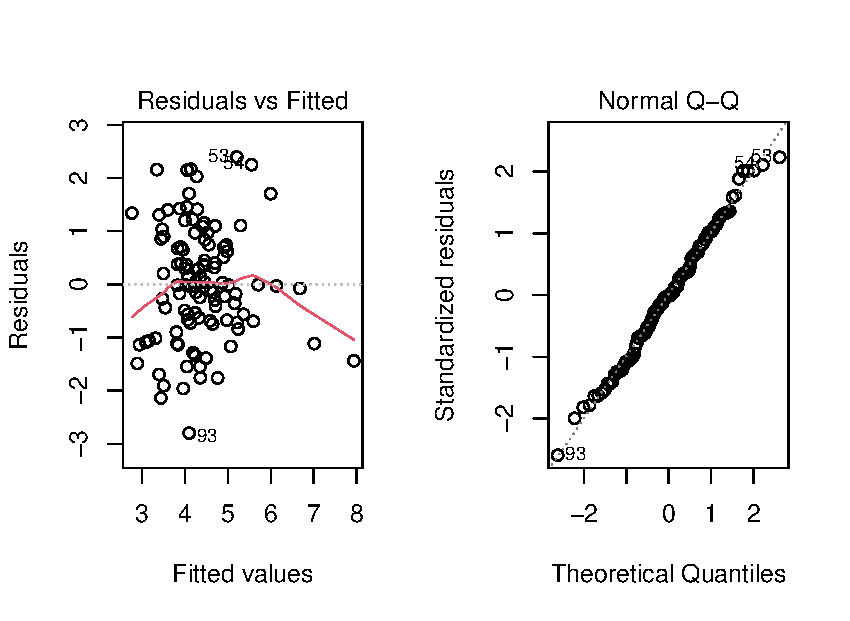
\includegraphics[width=1.0\textwidth]{fig/ex4-b.pdf}
\end{figure}
\emph{Explanation: 마찬가지로, 잔차들은 (a) \textbf{선형성}, (b) \textbf{독립성}: 특정한 패턴을 보이거나 (c) \textbf{등분산성}: 분산의 분포가 일정한 것으로 보아 가정을 위배한 것으로 보이지 않는다. 하지만 몇몇 잔차의 경우 범위를 벗어난 큰 값을 갖는 것으로 확인된다. 정규 분위수 그래프를 확인해 보면 양 끝쪽으로 직선에서 벗어난 점들이 관찰되는데 대부분의 잔차는 (d) \textbf{정규성}: 직선 주위에 몰려있는 것을 확인할 수 있다. 따라서 단순선형회귀모형의 적용은 타당함을 알 수 있다.} \\

\section*{Example 5}
다음의 데이터에 대하여 단순선형회귀식 $y=\alpha+\beta x$을 적합하고자 한다.

\begin{table}[htb!]
\centering
\begin{tabular}{|c|ccccccccccc|}
\hline
X & 0 & 1 & 3 & 3 & 5 & 7 & 8 & 8 & 10 & 11 & 13 \\ \hline
Y & 1 & 3 & 8 & 11 & 12 & 18 & 16 & 20 & 16 & 24 & 20 \\ \hline
\end{tabular}
\end{table}

\textbf{(a)} 두 변수 사이에 상관관계가 존재하는가? 표본 상관계수를 구하고 두 변수의 산점도를 그려라.
\begin{lstlisting}[style={r-style}]
X = c(0, 1, 3, 3, 5, 7, 8, 8, 10, 11, 13)
Y = c(1, 3, 8, 11, 12, 18, 16, 20, 16, 24, 20) 
df <- data.frame(X, Y)
cor(df$Y, df$X)
plot(Y ~ X, data=df)
\end{lstlisting}
\begin{lstlisting}[style={out-style}]
[1] 0.9197292
\end{lstlisting}
\begin{figure}[htb!]
    \centering
    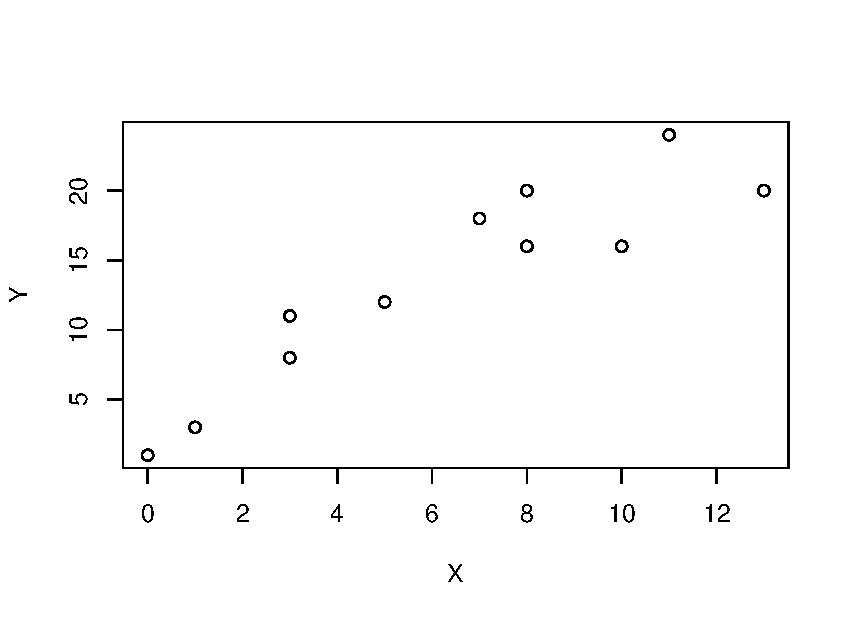
\includegraphics[width=0.6\textwidth]{fig/ex5-a.pdf}
\end{figure}
\emph{Explanation: 각각의 데이터 집합을 X 벡터와 Y 벡터에 대입 후 새로운 Dataframe에 저장한다. 이를 df라 정의하고 저장된 두 변수에 대한 상관계수를 구해보면 0.9197로 나타나고 plot()을 이용하여 그린 산점도를 통해 \textbf{두 변수 간에는 어느 정도 선형적 연관성이 있음}을 확인할 수 있다. } \\

\textbf{(b)} 두 변수 사이에 상관관계가 존재하는지 유의수준 5\% 수준에서 검정하여라.
\begin{lstlisting}[style={r-style}]
cor.test(df$Y, df$X)
\end{lstlisting}
\begin{lstlisting}[style={out-style}]
---------------------------------------------------------------------------------------
	Pearson's product-moment correlation

data:  df$Y and df$X
t = 7.0288, df = 9, p-value = 6.127e-05
alternative hypothesis: true correlation is not equal to 0
95 percent confidence interval:
 0.7135183 0.9793015
sample estimates:
      cor 
0.9197292 
---------------------------------------------------------------------------------------
\end{lstlisting}
\emph{Explanation: cor.test() 함수를 이용해 상관관계 유무를 검정한 결과, 검정통계량은 7.0288이고 유의확률은 매우 작은 것으로 확인되었다. 따라서 유의수준 5\%에서 두 변수 (X, Y) 사이의 상관관계가 존재한다는 매우 뚜렷한 증거가 있다.} \\

\end{document}
